%\input{/Users/joshyv/Research/misc/latex_paper.tex}
\documentclass{article}
\usepackage{amsmath}
\usepackage{graphicx}
\usepackage{amsfonts}
\usepackage{amssymb}
\usepackage{amsthm}
%\usepackage{cite}
\usepackage{algorithm}
\usepackage{algorithmic}
\usepackage{times}
\usepackage{fancyhdr}
\usepackage{graphicx}
\usepackage{verbatim}
\usepackage{color}
\pagestyle{fancy}

\oddsidemargin=0.0in %%this makes the odd side margin go to the default of 1inch
\evensidemargin=0.0in
\textwidth=6.5in
\headwidth=6.5in
\textheight=9in %%sets the textwidth to 6.5, which leaves 1 for the remaining right margin with 8 1/2X11inch paper
\headheight=12pt
\topmargin=-0.25in
%\headheight=0in
%\headsep=0in
%\pagestyle{headings}

\usepackage{hyperref}
% \usepackage{ulem}
% \usepackage{color}

% \newcommand{\loo}{$L^{(1)}_{h; \mD_n}$}
\newcommand{\conv}{\rightarrow}
% \newcommand{\Real}{\mathbb{R}}
% \providecommand{\tr}[1]{\textcolor{red}{#1}}

\newcommand{\mB}{\mathcal{B}}
\newcommand{\mD}{\mathcal{D}}
\newcommand{\mM}{\mathcal{M}}
\newcommand{\PP}{\mathbb{P}}           % probability
\newcommand{\EE}{\mathbb{E}}           % expected value
\newcommand{\II}{\mathbb{I}}           % expected value
\newcommand{\Real}{\mathbb{R}}           % expected value

\newcommand{\del}{\delta}
\newcommand{\sig}{\sigma}
\newcommand{\lam}{\lambda}
\newcommand{\gam}{\gamma}
\newcommand{\eps}{\varepsilon}

\providecommand{\mc}[1]{\mathcal{#1}}
\providecommand{\mb}[1]{\boldsymbol{#1}}
\providecommand{\mbb}[1]{\mathbb{#1}}
\providecommand{\mv}[1]{\vec{#1}}
\providecommand{\mh}[1]{\widehat{#1}}
\providecommand{\mt}[1]{\widetilde{#1}}
\providecommand{\mhc}[1]{\hat{\mathcal{#1}}}
\providecommand{\mhb}[1]{\hat{\boldsymbol{#1}}}
\providecommand{\mvb}[1]{\vec{\boldsymbol{#1}}}
\providecommand{\mtb}[1]{\widetilde{\boldsymbol{#1}}}

\newcommand{\argmax}{\operatornamewithlimits{argmax}}
\newcommand{\argmin}{\operatornamewithlimits{argmin}}


% \newcommand{\mN}{\mathcal{N}}

\newcommand{\hL}{\widehat{L}}
\newcommand{\MeB}{\mM \overset{\varepsilon}{{\sim}}_F \mB}
\newcommand{\MsB}{\mM \overset{S}{\sim}_F \mB}
\newcommand{\MnoteB}{\mM \overset{\varepsilon}{{\not\sim}}_F \mB}
\providecommand{\tr}[1]{\textcolor{black}{#1}}
\providecommand{\norm}[1]{\left \lVert#1 \right  \rVert}
\newcommand{\T}{^{\ensuremath{\mathsf{T}}}}           % transpose

\newtheorem{defi}{Definition}
\newtheorem{thm}{Theorem}
\newtheorem{thex}{Thought experiment}
\lhead{Vogelstein JT, et al}
\rhead{Neurocognitive Graph Theory}

\title{Are mental properties supervenient on brain properties?}

\author{Joshua T. Vogelstein$^1$, R. Jacob Vogelstein$^{1,2}$, Carey E. Priebe$^1$\\
$^1$Department of Applied Mathematics and Sciences, \\ Johns Hopkins University, Baltimore, MD, 21218,\\ $^2$National Security Technology Department, \\ Johns Hopkins University Applied Physics Laboratory, Laurel, MD 20723}

\begin{document}

\maketitle
%\tableofcontents
\begin{abstract}

	The ``mind-brain supervenience'' \tr{conjecture} suggests that all mental properties (e.g.\ consciousness, intelligence, personality, etc.) are derived from the physical properties of the brain. The validity of this \tr{conjecture} has been argued in philosophical terms for over 2,500 years. \tr{Alternative conjectures, including various non-physical causes of mental properties, seem rather implausible to many, but proving or disproving these alternatives has remained elusive.}  

	To address the question of whether the mind supervenes on the brain through empirical means, here we frame a supervenience hypothesis in rigorous mathematical terms and propose a modified version of supervenience (called $\varepsilon$-supervenience) that is amenable to scientific methods and statistical analysis. To elucidate this approach, we posit a thought experiment that illustrates how the probabilistic theory of pattern recognition can be used to make a one-sided determination of $\varepsilon$-supervenience. The physical property of the brain employed in this analysis is the graph describing brain connectivity (i.e., the \emph{connectome}), and $\varepsilon$-supervenience allows us to determine whether a particular mental property can be inferred from one's connectome to within any given misclassification rate $\varepsilon > 0$, regardless of the relationship between the two. In addition to the theoretical results, we show via simulation that given reasonable assumptions about class conditional probabilities and the amount of data available, the thought experiment can actually be conducted on a simple organism, \emph{Caenorhabditis elegans}, with currently available technology.

	The potential significance of this work can be divided into distinct disciplines.  To the philosopher, this work demonstrates that philosophical conjectures can be morphed into statistical hypotheses, amenable to experimental investigations, allowing the philosopher to add empirical support to their rational arguments.  To the statistician, herein lies the first proof to our knowledge of the existence of a universally consistent classifier on graphs, and a constructivist one at that.  To the neuroscientist, a theoretically possible experiment is proposed to garnish support for a hypothesis that is widely believed: that mental properties supervene on brain properties.


\end{abstract}

\vspace*{0.5 in}


\section{Introduction}

Questioning the relationship between the mind (thoughts, beliefs, preferences, emotions, intelligence, etc.) and the brain (the physical structure inside our skulls) dates back at least as far as 400~BCE, when Plato wrote the dialogues, in which he posited immateriality of the soul \cite{Plato97}. Approximately two millennia passed before these ideas reached their canonical form through Descartes's discussion of mind-body dualism \cite{Descartes1641}. Then, in the 20th century, Donald Davidson stated and popularized the mind-brain supervenience \tr{conjecture}, which claims that an agent cannot alter in some mental property without altering in some physical property \cite{Davidson70}. Contemporary fields of neural network theory and neuroscientific inquiry often assume mind-brain supervenience, or an even stronger assumption about mind-brain causality, but no previously proposed notion of supervenience seems amenable to empirical investigation. Here we define new versions of supervenience that formulate the \tr{conjecture} in rigorous mathematical terms and that can be experimentally tested \tr{as a hypothesis}.

\tr{The primary contributions of this work are as follows.  First, a notion of supervenience amenable to empirical investigation is formally introduced.  This renders the mind-brain dualism debate a hypothesis, rather than an assumption.  Second, in addition to expanding the space of questions amenable to hypothesis testing, we also demonstrate the limits of hypothesis testing.  Third we posit a very general model of brains and their associated mental properties that admits statistical analysis in a graph theoretical and statistical framework.  Fourth, we prove that this formulation admits a universally consistent classifier that is guaranteed to find the relationship between minds and brains, if one exists.  Fifth we demonstrate through simulation that the proposed universally consistent classifier has reasonable convergence properties on simulated brain-graph data.}


\section{Preliminaries} % (fold)
\label{sec:preliminaries}

The intention in this work is to develop greater insight regarding the relationship between minds and brains, using statistical methods, with particular interest in notions of supervenience.  We therefore first define the objects of interest, that is, minds and brains.

Let $b$ correspond to an agent's brain, which is a particular element from the set of all possible brains, $\mB$.  The set of possible brains $\mB$ is completely unrestricted, meaning that $\mB$ could be an infinite set, with arbitrarily complexity.  In particular, $b$ might represent the position, momentum, and type of each subatomic particle residing within the skull some agent.  Thus, each different $b \in \mB$ corresponds to some difference in the position, momentum, or type of at least one subatomic particle composing the brain.

Similarly, let $m$ correspond to an agent's mind, which is a particular element from the set of all possible minds, $\mM$.  The set of possible minds $\mM$ is also unrestricted. In particular, $m$ might represent all an agent's thoughts, beliefs, and preferences. Thus, each different $m \in \mM$ corresponds to a difference in at least one thought, belief, or preference. 


The mind-brain supervenience conjecture, is a relation between these two sets, the set of mental states and the set of brain states.  Donald Davidson canonized this conjecture in 1970 with the following quote: \cite{Davidson70}
\begin{quotation}
\noindent supervenience might be taken to mean that there cannot be two events alike in all physical respects but differing in some mental respect, or that an object cannot alter in some mental respect without altering in some physical respect,
\end{quotation}
can be concisely and formally stated: $m \neq m' \implies b \neq b' \, \forall (b,m), (b',m') \in \mB \times \mM$.  While mind-brain supervenience is a relatively strong claim, importantly, one can imagine far stronger relations, such as the following.

First, it may be the case that minds supervene on brains, but one cannot form an \emph{injective} relation from brains to minds.  An injective relation is any relation that preserves distinctness.  Thus if minds are injective on brains, then $b\neq b' \implies m \neq m' \, \forall (b,m), (b',m') \in \mB \times \mM$ (note that the directionality of the implication has been switched relative to supervenience). For instance, it might be the case that a brain could change without the mind changing.  Consider the case that a single subatomic particle shifts its position by a Plank length, changing brain state from $b$ to $b'$.  It is possible that the mental state supervening on brain state $b$ remains $m$, even after $b$ changes to $b'$.  In such a scenario, the mind might still supervene on the brain, but the relation from brains to minds is not injective. This argument also shows that supervenience is not necessarily a \emph{symmetric} relation.  Minds supervening on brains does not imply that brains supervene on minds.  

% In this case, it would be said that both $M$ supervenes on $B$ and $B$ supervenes on $M$. But it is not necessarily the case that if supervenience holds in one direction that it does or does not hold in the other direction.

Second, it may be the case that minds supervene on brains, but that brains do not cause minds.  For instance, consider an analogy where $M$ and $B$ correspond to two coins being flipped, each possibly landing on heads or tails.  Further assume that every time one lands on heads so does the other, and every time one lands on tails, so do the other. This implies that $M$ supervenes on $B$, but assumes nothing about whether $M$ causes $B$, or $B$ causes $M$, or some exogenous force causes both.  

% Supervenience is also not \emph{causality}.  Consider the coin flip example.  Nowhere did the notion of causality even arise.  It could be the case that $M$ causes $B$, or $B$ causes $M$, or some exogenous force causes both.  Thus, supervenience does not imply causality.  

Third, supervenience does not imply \emph{identity}.  Consider, for example, acceleration and velocity.  Clearly, acceleration supervenes on velocity, as acceleration cannot change without velocity changing (assuming one does not consider gravity as acceleration).  Similarly, velocity supervenes on position, as velocity cannot change without position changing.  Therefore, acceleration supervenes on position, by the transitive property of supervenience, but it is not the case that a change in acceleration is equal to a change in position.  Rather, position can change with constant velocity, meaning without acceleration changing.  

What supervenience does imply, however, is the following.   Imagine finding two different minds.  If $\MeB$, then the brains subvening under those two minds must be different.  In other words, there cannot be two different minds, either of which could supervene on a single brain.  Figure \ref{fig:rel} shows several possible relations between the sets of minds and brains.

\begin{figure}[htbp]
	\centering
		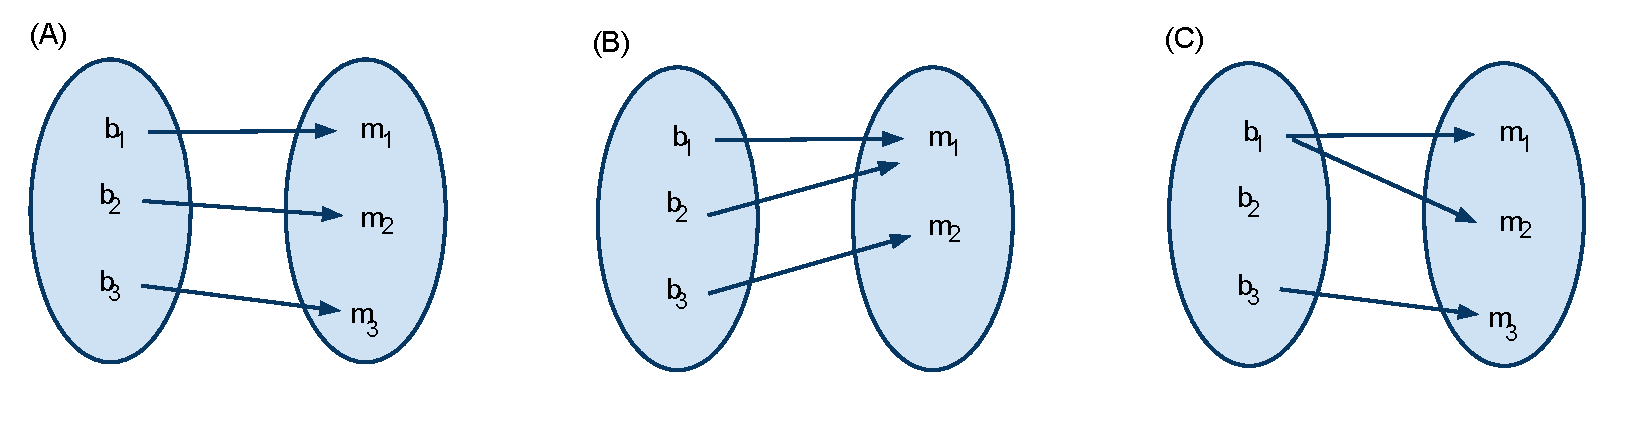
\includegraphics[width=1\linewidth]{supervenience_relations.pdf}
	\caption{Possible relations between minds and brains.  (A) Minds supervene on brains, and it so happens that there is a bijective relation from brains to minds.  (B) Minds supervene on brains, and it so happens that there is a surjective relation from brains to minds. (C) Minds are \emph{not} supervenient on brains, because two different minds supervene on the same brain.}
	\label{fig:rel}
\end{figure}


All of the above relations are \emph{logical} relations, not probabilistic relations. To facilitate both statistical analysis and empirical investigation, we project this supervenience notion into a statistical setting.  To proceed, we first define a \emph{model}, $\PP[B,M]=F_{BM}$, which specifies the probability of any element $(b,m)$ occurring from the space of all possible elements $\mB \times \mM$ (also called the \emph{sample space}).  The model could in theory come from any possible joint distribution defined on the sample space, $F_{BM} \in \mc{F}$, meaning that we only assume that it conforms to the \emph{probability axioms}:
\begin{enumerate}
	\item $0 \leq \PP[B=b,M=m] \leq 1$ for all $(b,m) \in \mM \times \mB$
	\item $\PP[\Omega]=1$ and $\PP[\emptyset]=0$, where $\Omega$ is the whole sample sample, that is, all elements, $(b,m) \in \mB \times \mM$
	\item any countable sequence of pairwise disjoint elements, $(b_1,m_1), (b_2,m_2), \ldots$ satisfies \\
	\mbox{$\PP[(b_1,m_1) \cup (b_2,m_2) \cup \ldots] = \sum_i \PP[(b_i,m_i)]$}.
\end{enumerate}
Given a model, one can then calculate any marginal or conditional distributions as a function of the model.  For instance, $\PP[B]=\int_{m \in \mM} \PP[B,M]\text{d}m$, or $\PP[M|B]=\PP[B,M]/\PP[B]$.  Given the definition of a model, statistical supervenience can be defined as follows:
\begin{defi}
\label{def1} 
$\mM$ is said to \textit{statistically supervene} on $\mB$ for distribution $F=F_{BM}$, denoted $\mM \overset{S}{\sim}_F \mB$, if and only if $\PP[m \neq m' | b=b']=0 \, \forall (b,m), (b',m') \in \mB \times \mM$. Alternately, $\MeB$ can be written as $\PP[m = m' | b = b']=1  \, \forall (b,m), (b',m') \in \mB \times \mM$.
\end{defi}
Statistical supervenience is therefore a probabilistic relation on sets.  Note that statistical supervenience is distinct from statistical correlation.  \emph{Statistical correlation} between brain states and mental states is defined as $\rho_{BM}=\EE[(B-\mu_B)(M-\mu_M)]/(\sig_B \sig_M)$, where $\mu_X$ and $\sig_X$ are the mean and variance of $X$, and $\EE[X]$ is the expected value of $X$.  If $\rho_{BM}=1$, then both $\MeB$ and $\mB \overset{S}{\sim}_F \mM$. Thus, correlation implies supervenience, but supervenience does not imply correlation.  


 % Consider the following analogy: one desires to understand the relationship between height and weight.  In such a scenario, height, $h$, could be assumed to be an element from the set of all possible heights, $\mc{H}=(0,\infty)$ cm; and weight, $w$, could be assumed to be an element from the set of all possible weights, $\mc{W}=(0,\infty)$ kgs.   Then, it may be assumed that an agent's height and weight is sampled identically and independently from some \emph{model}, that is $(h,w)\overset{iid}{\sim}\PP[H,W]=F_{HW}$. To gain insight into $F_{HW}$, one might then state hypotheses, collect data, and perform analyses.  Implicit in the exposition of a model is that both objects, height and weight here, are \emph{random objects}.  Note that this does not imply anything in particular about the distribution (which could be a point mass, for instance); rather, it is a formal definition necessary for statistical analysis and empirical investigation. 


% section preliminaries (end)

\section{Results}

\subsection{Theoretical results} % (fold)
\label{sub:theoretical_results}

% subsection theoretical_results (end)
If minds statistically supervene on brains, $\MsB$, then two different minds must supervene on two different brains.  This means that there exists a unique mapping from each brain to a single mind.  In other words, one can in principle construct a function $g(b): \mB \mapsto \mM$, that is a deterministic mapping from brains to minds.  It may be the case that subsets of brains from equivalence classes, such that any brain in that subset is mapped to the same mind (see, for example, $b_1$ and $b_2$ in Figure \ref{fig:rel}(A)).  Assuming for the moment that the space of all possible minds is finite, that is $| \mM| < \infty$, then we call any such function a \emph{classifier} (this assumption will later be relaxed).  Let $\mh{m}$ denote the output of a classifier, $g(b)=\mh{m}$.  Define misclassification rate as:
\begin{align}
	L_F(g) = P_{F}[g(B) \neq M] = \frac{1}{|\mB| |\mM|}\iint \II\{g(b)\neq m\} \text{d}b \text{d}m
\end{align}
where $\II\{\cdot\}$ indicates the indicator function, taking value one if its argument is true, and zero otherwise.  $L_F(g)$ therefore effectively counts the fraction of time $g$ misclassifies $b$. The Bayes optimal classifier $g^*$ minimizes $L_{F}(g)$ over all classifiers, that is
\begin{align}
	g^* = \argmin_{g \in \mc{G}} L_F(g)
\end{align}
where $\mc{G}$ is the set of all possible classifiers.  Thus, the \emph{Bayes error}, or Bayes risk, $L_F(g^*)$ is the minimum possible misclassification rate. The primary result of casting supervenience is a statistical framework is the following theorem: 
\begin{thm}
\label{thm1} 
$\mM$ is said to \textit{statistically supervene} on $\mB$ for distribution $F=F_{BM}$, denoted $\mM \overset{S}{\sim}_F \mB$, if and only if $L_{F}(g^*) = 0$.
\end{thm}
% \begin{thm} 
% 	\label{thm1} 
% 	Statistical supervenience implies that there exists a classifier that is \emph{always correct}, that is, $g(b)=m$, for all $(b,m) \in \mB \times \mM$.  
% \end{thm}

\noindent If minds supervene on brains, then, by the definition of supervenience, there exists a function that maps each brain deterministically to a particular mind.  This means that one could draw a decision boundary between all equivalence classes of brains, each class corresponding to a different mind, and no mind will reside within two different equivalence classes.  Thus, the optimal classifier would correctly find these decision boundaries, and therefore have no opportunity to err. $\square$

This relationship between statistical supervenience and Bayes error can therefore be described concisely: \mbox{$\MsB \Leftrightarrow L_F(g^*)=0$}.  Thus, the above arguments shows (for the first time to our knowledge) that statistical supervenience and zero Bayes error are equivalent. Further, statistical supervenience can be thought of as a constraint on the possible models.  Specifically, let $\mc{F}_s \subset \mc{F}$ be subset of models for which supervenience holds.  Then, $\mc{F}_s = \{F | L_F(g^*)=0\} \subset \mc{F}$.


\subsection{Hypothesis testing} % (fold)
\label{sub:hypothesis_testing}

While the above theorem is of potential theoretical interest, because the arguments rest on knowing $F_{BM}$ and $g^*$, which are typically unknown, they are pragmatically useless.  However, both $F_{BM}$ and $g^*$ could be estimated from data.  Let $(b_1,m_1), (b_2,m_2), \ldots, (b_n,m_n)$ be random samples taking their values in $\mB \times \mM$, independently and identically distributed according to model $F_{BM}$.  Generalizing the concept of a classifier $g$ to allow incorporation of training data, consider $g_n:\mB \times (\mB \times \mM)^n \mapsto \mM$ which takes as input an observed brain connectivity structure $b$ and $n$ training pairs $\tr{\mc{T}_n=}\{(b_1,m_1),\cdots,(b_n,m_n)\}$ and produces a classification $g_n(b;\tr{\mc{T}_n})=\mh{m}$.  Misclassification rate for this classifier will therefore be a random variable, because the training data $\mc{T}_n$ are random samples.  Therefore, instead of calculating misclassification rate for $g_n$, we compute the expected misclassification rate: % as the expectation of $\PP[g_n(B)=M | \mc{T}_n]$ over all possible training data corpuses:
\begin{align}
\EE[L_{F}(g_n)] = \EE[P_{F}[g_n(B;\tr{\mc{T}_n}) \neq M|\tr{\mc{T}_n}]] = \int \PP_F[g_n(B)=M | \mc{T}_n] \PP[\mc{T}_n] d\mc{T}_n.
\end{align}
Unfortunately, in practice, computing $\EE[L_F(g_n)]$, requires integrating over all possible training data corpuses, and by definition, we only have access to a single training data corpus.  We therefore define ``hold out'' misclassification performance:
\begin{align}
\EE[L_F(g_n)] %= \int \PP_F[g_n(B)=M | \mc{T}_{n'-n}] \PP[\mc{T}_{n'-n}] d\mc{T}_{n'n} \nonumber \\ 
&\approx  \hL^{n'}_{F}(g_n) = \sum_{\mc{T}_{n-n'}} \PP_F[g_n(B)=M | \mc{T}_{n-n'}] \PP[\mc{T}_{n-n'}],
\end{align}
where $n'<n$ is the number of held-out training samples, and the sum is taken over a sufficiently large number of subsets, $\mc{T}_{n-n'}$, such that $\hL^{n'}_F(g_n)$ converges.   $n' \hL^{n'}_{F}(g_n)$ is the expected number of misclassified minds, and has a binomial distribution, because for any of the $n'$ held-out samples, the classifier could be either correct or incorrect, thus $n' \hL^{n'}_{F}(g_n) \sim \text{Binomial}(n',L_{F}(g_n))$.

Before explicitly considering the problem of testing for statistical supervenience, we define a relaxed notion of supervenience:
\begin{defi}
\label{def2}
Given $\varepsilon > 0$, $\mM$ is said to $\varepsilon$-\textit{supervene} on $\mB$ for distribution $F=F_{BM}$, denoted $\MeB$, if and only if $L_{F}(g^*) < \varepsilon$.
\end{defi}

Given this relaxation, consider the problem of testing for $\eps-$supervenience.  First, specify a significance level, $\alpha$, such that if the p-value is less than $\alpha$, then the null is rejected.  Because we hope to reject the null, in favor of the alternative, let the null hypothesis be $H_0$: $L_{F}(g_n) \geq \eps$, and the alternative hypothesis be $H_A$: $L_{F}(g_n) < \eps$.  We reject for low values of the test-statistic, $n' \hL^{n'}_{F}(g_n)$.  Specifically, if $n' \hL^{n'}_{F}(g_n)$ is less than the critical value,  $c_{\alpha}(n',\varepsilon)$, then we reject.  The critical value is available under the least favorable distribution $\text{Binomial}(n',\varepsilon)$.  Thus, if $n' \hL^{n'}_{F}(g_n) < c_{\alpha}(n',\varepsilon)$, we can conclude with $100(1-\alpha$)\% confidence that $\MeB$.  The definition of $\eps$-supervenience therefore admits, for the first time to our knowledge, a statistical test of supervenience, given a specified $\eps$ and $\alpha$. Similar to the above, one can define the set of $\eps$-supervenience models as the set of models under which $\eps$-supervenience holds, that is: $\mc{F}_\eps = \{F | L_F(g^*)< \eps\}$.  One could then sort  $\eps$-supervenience subsets,  $\mc{F}_s \subseteq \mc{F}_{\eps} \subseteq \mc{F}_{\eps'} \subseteq \mc{F}$, for any $\eps < \eps'$.

% subsection hypothesis_testing (end)

\subsection{Power and consistency} % (fold)
\label{ssub:power_and_consistency}


Importantly, the utility of any statistical test depends both on the p-value, the probability of obtaining a test statistic at least as extreme as the observed value, and its power, the probability that the test will reject a false null hypothesis (in other words, the probability that it will not make a Type II error).  Ideally, the power of this test would go to unity, as $n,n' \rightarrow \infty$.  A sufficient condition for power to approach unity is that $g_n$ is a \emph{consistent} classifier.  A classifier is consistent if and only if its expected misclassification rate converges to the Bayes optimal limit with sufficient data, that is $\EE[L_F(g_n)] \conv L_F(g^*)$ as $n\conv \infty$. As the notation suggests, consistency of a classifier is a function of the true model, $F$.  Without any prior knowledge of what the model might be, one desires a \emph{universally consistent} classifier, that is a classifier that is consistent for all $F \in \mc{F}$.  

Unfortunately, the rate of convergence of $L_{F}(g_n)$ to $L_{F}(g^*)$ depends on the (unknown) distribution $F=F_{BM}$ \cite{DGL96}. Furthermore, arbitrarily slow convergence theorems regarding the rate of convergence of $L_{F}(g_n)$ to $L_{F}(g^*)$ demonstrate that there is no universal $n,n'$ which will guarantee that the test has power greater than any specified target $\beta > \alpha$ \cite{Devroye83}. For this reason, the test outlined above can provide only a one-sided conclusion: if we reject we can be $100(1-\alpha)$\% confident that $\MeB$ holds, but we can never be confident in its negation.  This means that we can never be confident that $\MeB$ does \emph{not} hold; rather, it may be the case that the evidence in favor of $\MeB$ is insufficient for any number of reasons, including that we simply have not yet collected enough data. Unfortunately, arbitrarily slow convergence theorems inform us that no matter how much data we collect, we cannot disambiguate between not yet having enough data, and $\MeB$ not holding.  Thus, without restrictions on $F_{BM}$, arbitrarily slow convergence theorems imply that our theorem of $\varepsilon$-supervenience does not \tr{strictly} satisfy Popper's {\it falsifiability} requirement \cite{Popper}. Given these limitations on even universal consistency, it is still the best one can hope for.  Therefore, we hope to obtain a universally consistent classifier to test for $\eps$-supervenience.

In 1977, Stone proved that a certain collection of $k_n$ nearest neighbor algorithms is universally consistent, assuming $b$ was a random $d$-dimensional vector $\mc{B} \subseteq \Real^d$ \cite{Stone77} (see Appendix \ref{app:knn} for an explanation of $k_n$ nearest neighbor algorithms, and constraints to ensure universal consistency).  This beautiful result would be directly applicable to mind-brain supervenience, if we were satisfied representing brains by random vectors.  However, brains are rich with structure, and therefore, other, more sophisticated data structures can better capture aspects of the brain that many of us believe to be true. Therefore, in the next section, we introduce the concept of a \emph{brain-graph}, which can have a much richer structure than a vector.  We then generalize the $k_n$ nearest neighbor algorithm to operate in this domain, and extend the universal consistency proof as well.


% subsubsection power_and_consistency (end)


\subsection{Brain-graphs} % (fold)
\label{sub:brain_graphs}

In 1891, H Waldeyer-Hartz first formally proposed the ``neuron doctrine'' \cite{Waldeyer-Hartz1891}, which states that the nervous system is a complex \emph{network} of ``neurons'' (a term invented in the above review), largely based on Ramon y Cajal's work using the Golgi stain \cite{Finger01}.  This doctrine has been central to much of the development of neuroscience and artificial intelligence for over 100 years.  


% subsection brain_graphs (end)


\section{Old results} % (fold)
\label{sec:old_results}

% (fold)
% Let $\mB$ be the observation space for some physical property, such as brain connectivity structure (i.e., connectome; see \cite{SpornsKotter05,LichtmanSanes08,Seung09}). Let $\mM$ be the (finite) indicator space for some mental property, such as knowing calculus. Thus, for $b \in \mB$ and $m \in \mM$, the pair $(b,m)$ represents a brain property/mind property pair.
% 
% %Let $\{(B_i,M_i)\}_{i=1}^n \overset{iid}{\sim} F_{BM}$
% Let $(B,M), (B_1,M_1),\cdots,(B_n,M_n)$ be random observation pairs taking their values in $\mB \times \mM$, independently and identically distributed according to some joint probability distribution $F=F_{BM}$. Abusing notation to conceptually identify the properties with their spaces, the statistical supervenience relation $\mM \overset{S}{\sim}_F \mB$ says that $M_i \neq M_j \implies B_i \neq B_j$ (almost surely; where $\implies$ does not suggest causation). That is, observing $B=b$ can allow us to assign $m$ to $M$. While previously proposed notions of mind-brain-supervenience claim that all mental properties supervene on physical properties \cite{Kim95}, here we consider empirically investigating only whether a particular mental property $\mM$ statistically supervenes on a particular physical property $\mB$.
% 
% Let $g:\mB \mapsto \mM$ be a classifier, which takes as input an observed brain connectivity structure $b$ and produces a classification $\widehat{m}=g(b)$ for the unobserved mental property $m$. The Bayes optimal classifier $g^*$ minimizes $L_{F}(g)$ over all classifiers, where $L_{F}(g) = P_{F}[g(B) \neq M]$ denotes the probability of misclassification for classifier $g$ under joint distribution $F=F_{BM}$. We can therefore rigorously define \textit{statistical supervenience}:
% 
% \begin{defi}
% \label{def1} 
% $\mM$ is said to \textit{statistically supervene} on $\mB$ for distribution $F=F_{BM}$, denoted $\mM \overset{S}{\sim}_F \mB$, if and only if $L_{F}(g^*) = 0$.
% \end{defi}
% 
% \tr{(Note that this definition does not imply a one-to-one mapping.)}  \tr{To allow for the possibility of only \emph{partial} supervenience,}  we relax the above statistical supervenience to define $\varepsilon$-\textit{supervenience}:
% 
% \begin{defi}
% \label{def2}
% Given $\varepsilon > 0$, $\mM$ is said to $\varepsilon$-\textit{supervene} on $\mB$ for distribution $F=F_{BM}$, denoted $\MeB$, if and only if $L_{F}(g^*) < \varepsilon$.
% \end{defi}
% 
% \tr{Unfortunately, in general $F$ is unknown, but can be estimated from the data. Therefore,} generalizing the concept of a classifier $g$ to allow consideration of training data, consider $g_n:\mB \times (\mB \times \mM)^n \mapsto \mM$ which takes as input an observed brain connectivity structure $b$ and $n$ training pairs $\tr{\vec{d}_n=}(b_1,m_1),\cdots,(b_n,m_n)$ and produces a classification $\widehat{m}=g_n(b;\tr{\vec{d}_n})$. Let $L_{F}(g_n) = E[P_{F}[g_n(B;\tr{\vec{D}_n}) \neq M|\tr{\vec{D}_n}]]$.
% 
% Consider the problem of testing for $\varepsilon$-supervenience. Let the null hypothesis be given by $H_0: L_{F}(g_n) \geq \varepsilon$ so that if we reject at level $\alpha >0$ in favor of the alternative hypothesis $H_A: L_{F}(g_n) < \varepsilon$ then we can conclude, with $100(1-\alpha$)\% confidence, that $\MeB$. Letting $\hL^{n'}_{F}(g_n)$ denote the hold-out estimate of misclassification performance based on $n'$ test observations, we note that $\hL^{n'}_{F}(g_n)$ is distributed $\text{Binomial}(n',L_{F}(g_n))$.
% 
% % section old_results
% 
% The test rejects for small $\hL^{n'}_{F}(g_n)$. The level $\alpha$ critical value $c_{\alpha}(n',\varepsilon)$ is available under the least favorable distribution $\text{Binomial}(n',\varepsilon)$. Furthermore, $\MeB$ implies $L_{F}(g^*) < \varepsilon$, and thus if $g_n$ is a {\it consistent} classifier for $F=F_{BM}$ --- that is, if $\lim_n L_{F}(g_n) = L_{F}(g^*)$ --- then the power of this test (the probability of rejecting when in fact the alternative is true) goes to unity as $n,n' \rightarrow \infty$. Thus we have an inference procedure: 
% 
% \begin{thm} 
% 	\label{thm1} 
% 	Given $\alpha > 0$, we can test $\MeB$ so that rejection implies $\MeB$ holds with probability greater than or equal to $1-\alpha$. Furthermore, given a consistent classifier the power of the test converges to unity. 
% \end{thm}
% 
% Since the joint distribution $F=F_{BM}$ is unknown, the utility of Theorem \ref{thm1} requires that $g_n$ be a {\it universally consistent} classifier --- that is, $\lim_n L_{F}(g_n) = L_{F}(g^*)$ for all distributions $F=F_{BM}$. Unfortunately, the rate of convergence of $L_{F}(g_n)$ to $L_{F}(g^*)$ depends on the (unknown) distribution $F=F_{BM}$ \cite{DGL96}. Furthermore, arbitrarily slow convergence theorems regarding the rate of convergence of $L_{F}(g_n)$ to $L_{F}(g^*)$ demonstrate that there is no universal $n,n'$ which will guarantee that the test has power greater than any specified target $\beta > \alpha$ \cite{Devroye83}. For this reason, the test outlined above can provide only a one-sided conclusion: if we reject we can be $100(1-\alpha)$\% confident that $\MeB$ holds, but we can never be confident in its negation. Thus, without restrictions on $F_{BM}$, arbitrarily slow convergence theorems imply that our theorem of $\varepsilon$-supervenience does not \tr{strictly} satisfy Popper's {\it falsifiability} requirement \cite{Popper}. Given these caveats, consider the following thought experiment:
% (end)


\begin{thex}
Let the physical property under consideration be brain connectivity structure (``connectome''), so $b$ is a graph \tr{(or, network)} with vertices representing neurons (or neuroanatomical regions) and edges representing connections between neurons (or white matter tracts). Further let $\mB$, the observation space, be the collection of all graphs on a finite number of vertices, and let $|\mB|$ be countable. Now, imagine collecting very large amounts of very accurate independent and identically distributed brain-graph data and the associated mental property indicators. A $k_n$-nearest neighbor classifier using an isomorphism-matching Frobenius norm is universally consistent (see Appendix 1 for proof). Therefore, Theorem \ref{thm1} applies and the existence of a universally consistent classifier guarantees that eventually (in $n,n'$) we will be able to conclude $\MeB$ for this mental/brain property pair, if indeed $\varepsilon$-supervenience holds. This logic holds for directed graphs or multigraphs or hypergraphs with discrete edge weights and vertex attributes. Furthermore, Appendix 1 also extends the proof to deal with other matrix norms (which might speed up convergence), and the regression scenario, where $|\mM|$ is infinite.  
\end{thex}

\section{Discussion}

While the above thought experiment addresses the question of $\varepsilon$-supervenience, it does not address causality. Assuming we have confirmed $\MeB$ for a particular mental/brain property pair with confidence level $\alpha$, then morphing the brain (by altering edges) could be used to determine whether the relation is in fact causal.

Practical issues regarding actually conducting the above thought experiment include: (1) as stated, we must consider the space $\mB$ to be the quotient space of graphs mod graph isomorphism, unless the vertices are {\it labeled}; (2) a more informative and tractable distance on $\mB$ may be desired, as the $k_n$-nearest neighbor classifier under our Frobenius norm (or other norm; see Appendix 1 for details) may have a rate of convergence so slow and a computational demand so high as to be impractical; and (3) collecting enough sufficiently accurate independent and identically distributed brain-graph data and the associated mental property indicators may be beyond current technological capabilities. Regardless, related experimental work includes collecting various types of brain graph data \cite{WhiteBrenner86, DenkHorstmann04, BriggmanDenk06} and various approaches to inference on brain graphs \cite{MackeBorst08, Mishchenko09, LuLichtman09}, suggesting feasibility of such an experiment in the near future (see Appendix 2 for a simulated example of a feasible experiment). Nevertheless, our thought experiment suggests that we can hope to determine that a given mental property under consideration $\varepsilon$-supervenes on a brain's connectivity structure. \tr{This thought experiment, together with (i) the formal definition of $\varepsilon$-supervenience, (ii) the brain-graph model, and (iii) the universal consistency proof on graphs, is the first \emph{proof} (to our knowledge) that empirically investigating supervenience is at least theoretically possible.}


% You may title this section "Methods" or "Models". 
% "Models" is not a valid title for PLoS ONE authors. However, PLoS ONE
% authors may use "Analysis" 
% \section{Materials and Methods}

\appendix
\section{$k_n$ nearest neighbor algorithm} % (fold)
\label{app:knn}


Assume that $b$ is a real $d$-dimensional vector, $b \in \mc{B} \subseteq \Real^d$, and $m$ is a binary indicator, $m \in \mc{M} = \{0,1\}$.  Then, further assume that we have observed a collection of training data, $\mc{T}_n =\{(b_i,m_i)\}_{i=1}^n$, each sampled identically and independently from some unknown joint distribution, $(b_i,m_i)\overset{iid}{\sim} F_{BM}$.  A new brain, $b$, called the ``test brain'', is then observed, and one desires to find the most likely class of the new brain, $m$.  The $1$-nearest neighbor classifier works as follows.  Compute the distance between the test brain and all the training brains, $d_i=d(b,b_i)$ for all $i \in [n]$, where $[n]=1,2,\ldots, n$.  Then, sort them, $d_{(1)} < d_{(2)} < \ldots < d_{(n)}$, where parenthetical indices, $(i)$, indicate rank order.  One can then also obtain a rank order for the training minds, $m_{(1)}, m_{(2)}, \ldots, m_{(n)}$, where $m_{(i)}$ is the class of the $i^{th}$ closest training brain to $b$.  The $1$ nearest neighbor algorithm predicts that the unobserved mind is of the same class as the closest brain's class: $m=m_{(1)}$.  The $k_n$ nearest neighbor is a straightforward generalization of this approach.  It says that the test mind is in the same class as which ever class is the majority class of the $k_n$ nearest neighbors, $m=\II\{\sum_{i=1}^{k_n} m_{(i)} > k_n/2\}$.  Given a particular choice of $k_n$ (the number of nearest neighbors to consider), and a choice of $d(\cdot,\cdot)$ (the distance metric used to compare the test datum and training data), one then has a relatively simple and intuitive algorithm.  

Unfortunately, no such algorithm is universally consistent.  Let $g_n$ be the $k_n$ nearest neighbor classifier when there are $n$ training points.  Then, a collection of such algorithms, $\{g_n\}$,  with $k_n$ increasing with $n$, can be universally consistent under certain constraints. In particular, as $n$ increases, $k_n$ must also increase, but not quite as quickly.  Formally, $k_n$ must satisfy: (i) $k_n \conv \infty$ as $n \conv \infty$ and (ii) $k_n/n \conv 0$ as $n\conv\infty$. In Stone' original proof, the $L_2$ norm ($d(b,b')=\sum_{j=1}^d (b_j-b_j')^2$, where $j$ indexes elements of the $d$-dimensional vector) was shown to satisfy the constraints on a distance metric for this collection of classifiers to be universally consistent.  Later, others extended these results to apply to any $L_p$ norm \cite{DGL96}.

This algorithm also readily generalizes to the $C$-way classification problem, where there $C \geq 2$ classes.  Instead of finding the majority class of the $k_n$ nearest neighbors, one instead finds the plurality class, that is, the class with the most training samples within the $k_n$ nearest neighbors.  This algorithm generalizes even further, when $\mc{M}$ is no longer discrete, but rather continuous, for instance, $\mc{M}=\Real$.  In such a scenario, this approach is called $k_n$ nearest neighbor \emph{regression}.

% section _k_n_nearest_neighbor_algorithm (end)



\section{$k_n$-nearest neighbor universal consistency for graphs}
\label{proof}

Assume first that all graphs are simple \tr{(meaning undirected with no loops and binary edges)}, on the same set of vertices, and that the graphs are labeled so that we know which vertex in one graph corresponds to which vertex in another. Then the Frobenius distance function $d(b_1,b_2)$ can be written in terms of the associated adjacency matrices $A_1$ and $A_2$: $d(b_1,b_2) = ||A_1-A_2||_F$. If the graphs are identical, then $d(b_1,b_2) = 0$, and if the graphs are different, then $d(b_1,b_2) \geq 1$. Since the space $\mB$ is finite, $n$ large enough guarantees that with probability approaching unity at least $k_n$ training samples coincide with each atom, so long as $k_n/n \rightarrow 0$. Then $k_n \rightarrow \infty$ guarantees that the nearest neighbor vote-winner for each atom will eventually coincide with Bayes' choice, yielding universal consistency.

In the foregoing argument, there exists a smallest non-zero atomic probability $p_{min}$, and ``$n$ large enough'' is driven by this probability. Generalizing to countable $\mB$ with discrete weights, we see that given $\delta > 0$, there is a finite set $S$ with $\PP[S]>1-\delta$ and smallest atomic probability $p_{min}$, so that $L_{F}(g_n) \rightarrow c \leq L_{F}(g^*) + \delta$, yielding universal consistency.

If the graphs may have different numbers of vertices, and are unlabeled, we consider the isomorphism-matching Frobenius norm. Assume without loss of generality that $b_1$ has at least as many vertices as $b_2$, and write $A_2^P$ for the adjacency matrix associated with $b_2$ ``padded'' to include extra isolated vertices so that $A_2^P$ is the same size as $A_1$. Then $d(b_1,b_2) = \min_Q ||Q A_1 Q^T - A_2^P||_F$ where the minimum is taken over all permutation matrices \cite{HornJohnson90}. Under the equivalence relation induced by this isomorphism-matching, the foregoing universal consistency argument holds.
%\tr{Trivially, this argument also applies to graphs with (self-) loops, and
%directed, colored, or weighted edges, and hypergraphs.}

Several points of note:  isolated vertices are ignored in our equivalence relation; the class-conditional signal is entirely encompassed by the connectivity structure; the graph isomorphism problem is computationally hard \cite{ConroyLouis97,ZaslavskiyVert08}; and the argument employed here does not capture the concept of ``nearness implies likelihood of similar class''---we simply rely on atomic behavior.

Finally, the above proof can be straightforwardly generalized to utilize any matrix norm, $\norm{b_1-b_2}_A=\norm{A(b_1-b_2)}$, assuming that $A A\T$ is positive definite (see \cite{DGL96} pg. 455 for proof when $b_i$'s are vectors).  Furthermore, we can relax the constraint that mental properties are finite, that is, we can allow any $|\mM| = \infty$ (see \cite{Stone77} for proof when $b_i$'s are vectors).  The proof for the case when $b$ is an adjacency matrix follows immediately upon first defining a bijective embedding of the matrix into a vector space, and then embedding each adjacency matrix in that space.  

%\appendix
\section{Simulation} \label{simulation}

As an example of a feasible experiment, one may consider a species whose nervous system consists of the same (small) number of labeled neurons for each organism. {\it Caenorhabditis elegans} is believed to be such a species \cite{Durbin87}. The hermaphroditic C.~elegans' somatic nervous system consists of 279 interconnected neurons. While the graph with these neurons as vertices and edges defined by chemical synapses between neurons is not identical across individuals, it is reasonably consistent \cite{Durbin87}. Furthermore, these animals exhibit a rich behavioral repertoire that depends on circuit properties \cite{deBonoMaricq05}. Thus, one may design an experiment by describing the joint distribution $F_{BM}$ via class-conditional distributions $F_{B|M=m_j}$ for the C.~elegans brain-graph for two mental properties of interest, $m_0$ and $m_1$, along with the prior probability of class membership $\PP[M=m_1]$. Here the mental property corresponds to the C.~elegans exhibiting or not exhibiting a particular behavior (e.g., response to an odor).

Simulations suggest that one may build a classifier, practically and with a manageable training sample size $n$, that demonstrates $\varepsilon$-supervenience with reasonable choices for $\varepsilon$ and $\alpha$ and a plausible joint distribution $F_{BM}$ (Figure \ref{fig1}). To generate the data, we let the class-conditional random variable $E_{ij} | M=m_0$ be distributed Poisson$(A_{ij}+\eta)$, where $A_{ij}$ is the number of chemical synapses between neuron $i$ and neuron $j$ according to \cite{VarshneyChklovskii09}, with noise parameter $0<\eta \ll 1$. The class-conditional random variable $E_{ij} | M=m_1$ is distributed Poisson$(A_{ij}+ \tr{z_{ij}})$ for neurons $i,j \in \mD$, where $\mD$ is the set of edges deemed responsible for odor-evoked behavior according to \cite{ChalasaniBargmann07}, with signal parameter $\tr{z_{ij}}$ uniformly sampled from $[-5,5]$. We consider $k_n$-nearest neighbor classification of labeled multigraphs (directed, with loops) on 279 vertices, under Frobenius norm. The $k_n$-nearest neighbor classifier used here satisfies $k_n \rightarrow \infty$ as $n \rightarrow \infty$ and $k_n/n \rightarrow 0$ as $n \rightarrow \infty$, ensuring universal consistency. (Better classifiers can be constructed for the joint distribution $F_{BM}$ used here; however, we demand universal consistency.)

\begin{figure}[!ht]
\centering 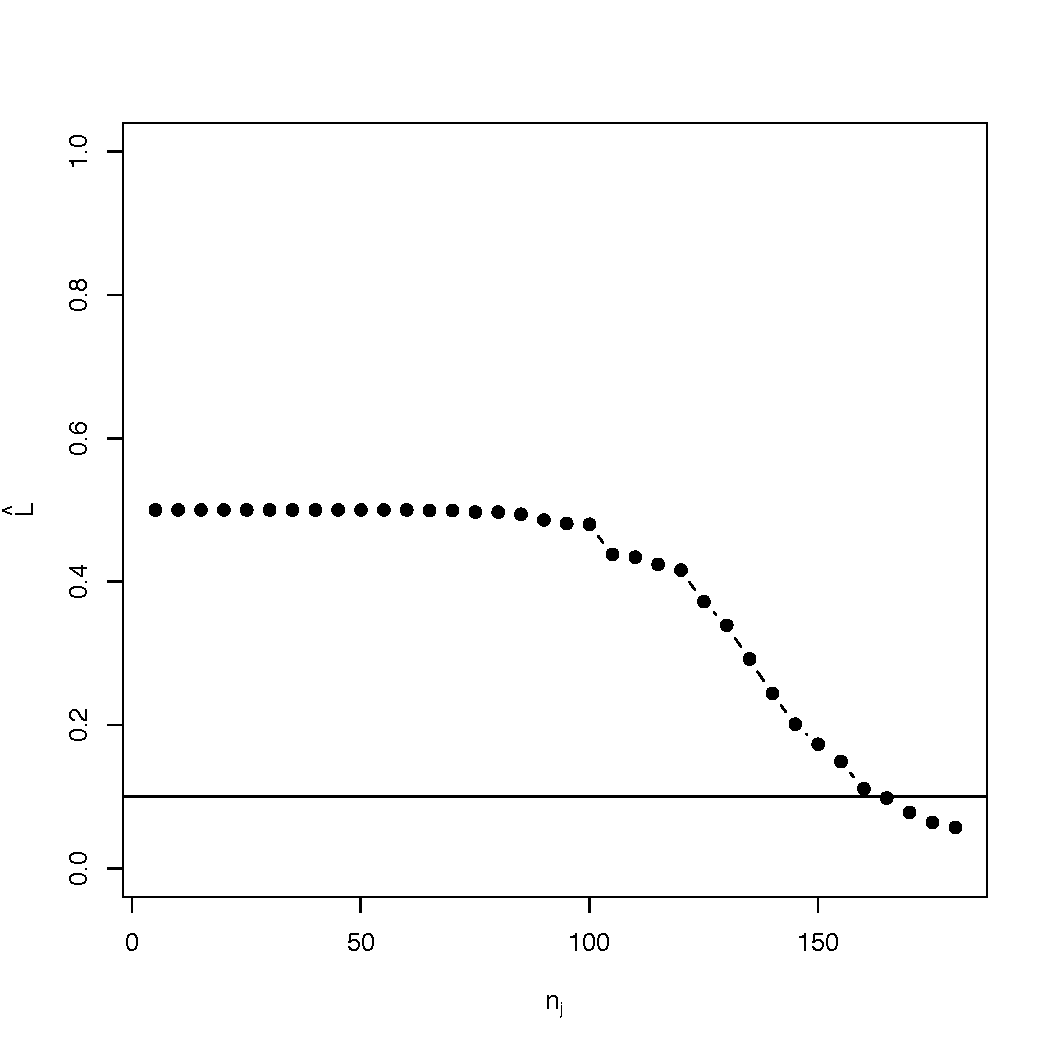
\includegraphics[width=.5\linewidth]{Lhatplot}
\caption{C.~elegans graph classification simulation results. $\hL^{1000}_{F}(g_n)$ is plotted as a function of class-conditional training sample size $n_j$, suggesting that for $\varepsilon=0.1$ we can determine that $\MeB$ holds with $99\%$ confidence with just a few hundred training samples generated from $F_{BM}$. Each dot depicts an estimate for $L_{F}(g_n)$; standard errors are $(L_{F}(g_n)(1-L_{F}(g_n))/1000)^{1/2}$\tr{; e}.g., $n_j = 180$ ; $k_n = 53$ ; $\hL^{1000}_{F}(g_n) = 0.057$; standard error less than 0.01. We reject $H_0: L_{F}(g^*) \geq 0.10$ at $\alpha=0.01$. $L_{F}(g^*) \approx 0$ for this simulation.
}
\label{fig1}
\end{figure}


Importantly, conducting this experiment {\it in actu} is not beyond current technological limitations. 3D superresolution imaging \cite{VaziriShank08} combined with neurite tracing algorithms \cite{HelmstaedterDenk08,Mishchenko09,LuLichtman09} allow the collection of a brain-graph within a day. Genetic manipulations, laser ablations, and training paradigms can each be used to obtain a non-wild type population for use as $M=m_1$ \cite{deBonoMaricq05}, and the class of each organism ($m_0$ vs.~$m_1$) can also be determined automatically \cite{BuckinghamSattelle08}.


% Do NOT remove this, even if you are not including acknowledgments
\section{Acknowledgments}

The authors would like to acknowledge helpful discussions with J Lande and B Vogelstein. 


% \section{References}
% The bibtex filename
\bibliography{biblist}
\bibliographystyle{ieeetr}

% \clearpage
% \section{Figure Legends}
% 
% Figure 1: C.~elegans graph classification simulation results. $\hL^{1000}_{F}(g_n)$ is plotted as a function of class-conditional training sample size $n_j$, suggesting that for $\varepsilon=0.1$ we can determine that $\MeB$ holds with $99\%$ confidence with just a few hundred training samples generated from $F_{BM}$. Each dot depicts an estimate for $L_{F}(g_n)$; standard errors are $(L_{F}(g_n)(1-L_{F}(g_n))/1000)^{1/2}$\tr{; e}.g., $n_j = 180$ ; $k_n = 53$ ; $\hL^{1000}_{F}(g_n) = 0.057$; standard error less than 0.01. We reject $H_0: L_{F}(g^*) \geq 0.10$ at $\alpha=0.01$. $L_{F}(g^*) \approx 0$ for this simulation.
% 



\end{document}

